\documentclass{beamer}
\usetheme{Copenhagen}
\usecolortheme{beaver}
\setbeamertemplate{navigation symbols}{}
\setbeamertemplate{footline}{\parbox[t][12pt][c]{12pt}{~\scriptsize\insertframenumber}}
% \usepackage{beamerthemesplit} // Activate for custom appearance

\title{Declarative Cartography}
\subtitle{In-Database Map Generalization of Spatial Datasets}
\author{Pimin Konstantin Kefaloukos, Marcos Vaz Salles, Martin Zachariasen}
\date{\today}

\begin{document}

\frame{\titlepage}

% MOTIVATION
\frame
{
  \frametitle{Motivation}
  \begin{itemize}
  \item Zoomable map based on vector data
  \item At lower scales: too many objects to fit the map
  \item Map should balance \emph{representation} and  \emph{legibility}~\footnote{This map of tourism POI has only representation, not legibility}
  \item We need \emph{generalization}
  \end{itemize}

  \fbox{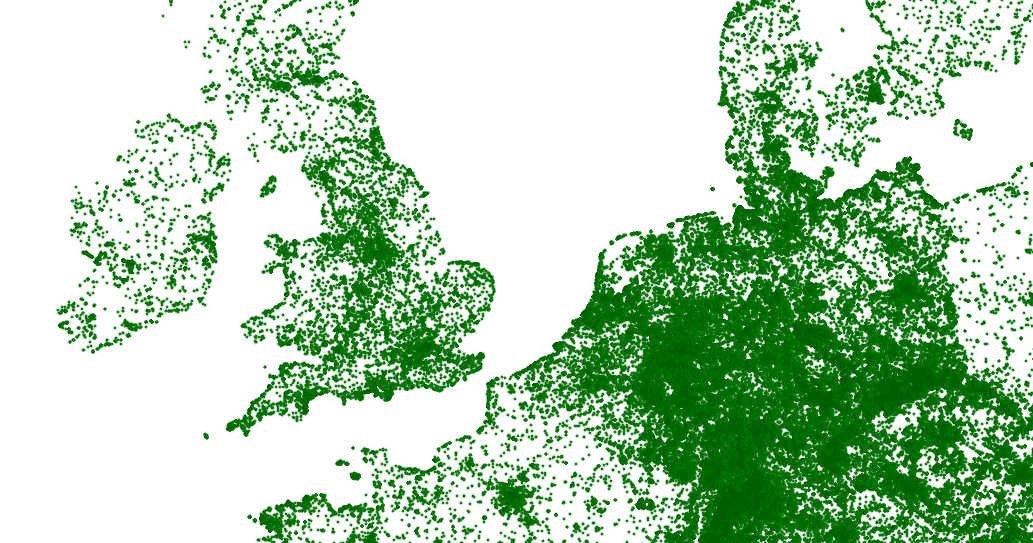
\includegraphics[scale=0.23]{figs/toomanyobjects.png}}
}

\frame
{
  \frametitle{Conflicts}
  \emph{Different pieces of information have to '{fight}' for their representation in a specific level of detail - Monika Sester}
  
  \begin{center}
  	\fbox{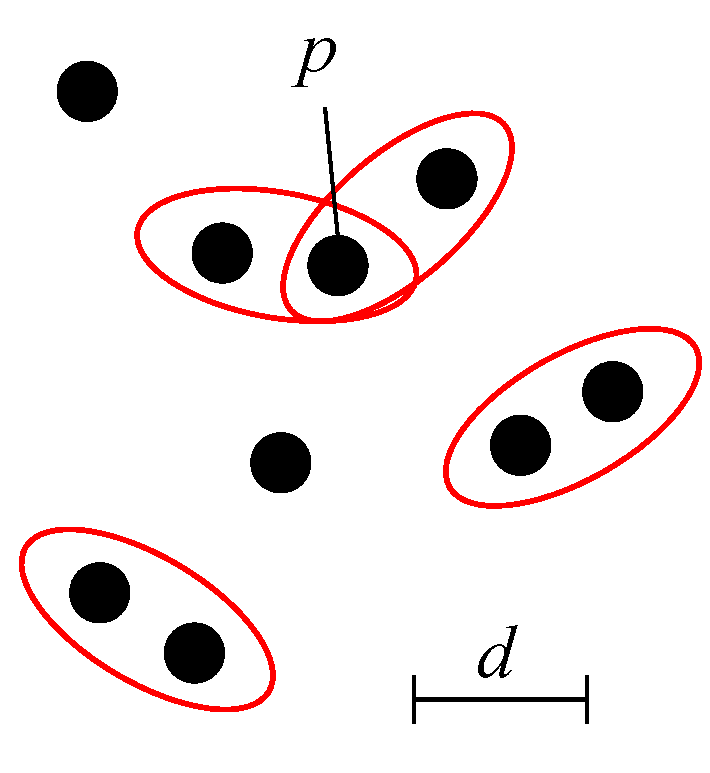
\includegraphics[scale=0.20]{figs/cvl_proximity_conflicts.pdf}}
  \end{center}
  
  \begin{itemize}
  \item Model fighting as a set of \emph{conflicts}
  \item A conflict is subset of records, that violate a \emph{constraint} on zoom-level $z$, for example a \emph{proximity constraint}
  \item Resolve conflict: Choose records that are filtered out
  \end{itemize}
}

% OPTIMIZATION
\frame
{
  \frametitle{Modelling}
  \begin{itemize}
  \item Record $r \in R$ has '{importance}' $w_r$ (for example star-rating of restaurant)
  \item 0-1 variable $x_{rz}$ : $1$ if record $r$ is \emph{filtered out} on zoom-level $z$
  \item 
  \end{itemize}
}


% APPROACH
\frame
{
  \frametitle{Model}
  \begin{itemize}
  \item Set of objects $R$
  \item $\mathcal{Z}$ zoom levels: $\lbrace 1, \dots, \mathcal{Z} \rbrace$
  \item 0-1 decision variable $x_{rz}$ for each record $r \in R$ and each zoom level $z \in \lbrace 1, \dots, \mathcal{Z} \rbrace$; this decision variable is 1 if record $r$ is \emph{filtered out} on zoom level $z$.
    \item Each object $r \in R$ has a weight $w_r$ (importance of object)
  \end{itemize}
}


% LANGUAGE
\frame
{
  \frametitle{Language}
}

% MODEL
\frame
{
  \frametitle{Model}
}

% RELATED WORK
\frame
{
  \frametitle{Related work}

  \begin{itemize}
  \item \emph{Efficient Spatial Sampling of Large Geographical Tables}. Das Sarma, A., Lee, H., Gonzalez, H., Madhavan, J., \& Halevy, A. (2012).
  \item \emph{Generalization of land cover maps by mixed integer programming}. Haunert, J.-H., \& Wolff, A. (2006). 
  \item \emph{Automated map generalization with multiple operators: a simulated annealing approach}. Ware, J. M., Jones, C. B., \& Thomas, N. (2003).
  \item \emph{Constant information density in zoomable interfaces}. Woodruff, A., Landay, J., Stonebraker, M. (1998).
  \item \emph{Retrieval of Information from Complex Alphanumeric Displays: Screen Formatting Variables� Effects on Target Identification Time}. Springer, C. J. (1987). 
  \end{itemize}
}


\end{document}
